\section{Results and Future Work}
We got the best results with batch size- 128, learning rate- 0.001, dropout- 0.5, num\_layers- 2, activation function- sigmoid, optimizer- adam. The model trained over undersampled data performs poorly over the test data when compared with the model trained over SMOTE sampled data. We were able to achieve 0.95 f1- score performance for majority class and 0.57 f1-score performance for minority class i.e. insincere questions on the test data using these parameters, where the input data fed to the model is sampled used SMOTE.  For the model trained over undersampled data, we get an f1-score of 0.93 for the majority class 0.48 for the minority class.
\begin{figure}[h]
	\begin{center}
		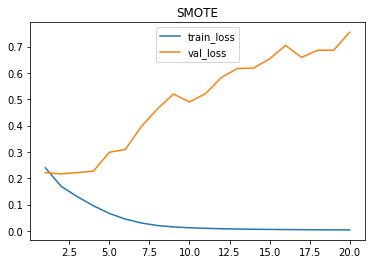
\includegraphics[width=150pt]{figures/smote.png}
		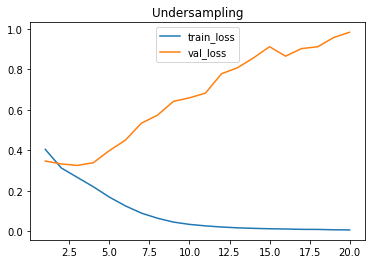
\includegraphics[width=150pt]{figures/undersampling.png}
		\label{fig:Model Performance over SMOTE}
	\end{center}
\end{figure}

Whereas, the existing Model 1 got a F1-score of 0.65 without using any embeddings with activation function- sigmoid, optimizer-adam and metrics- accuracy and the best F1-score of 0.67 using Glove embedding in Model 2. The existing model performed better than our proposed model as it used Gated Recurrent Unit (GRU) which performs better than Long short-term memory (LSTM) used in our model, as GRU is easy to modify and doesn't require memory units, so it trains faster and is much more efficient than LSTMs.

An extension or improvement of our work would be to leverage an attention model to identify which parts of the sequences are holding high information that can help predict the correct class. Also, models using Gated Recurrent Unit (GRU) have shown promising results in identifying the classes with high accuracy and can be used in combination with attention mechanism to achieve better results. 